
\section{Sensitivity analyses}
\subsection{Sensitivity analysis using alternative base mixing matrices}
We ran an alternative sensitivity analysis using the mixing matrices from Prem et al. 2020,\cite{RN81} which is currently available as a pre-print, rather than those from the 2017 publication. The results of this analysis were similar to that of the baseline analysis and are presented in Figure \ref{fig:prem_sensitivity_outputs}, Figure \ref{fig:prem_sensitivity_key_params} and Figure \ref{fig:prem_sensitivity_epi_params}. These results show no significant epidemiological differences from those derived from the base case analysis.

\begin{figure}[ht]
    \resizebox{1\textwidth}{!}{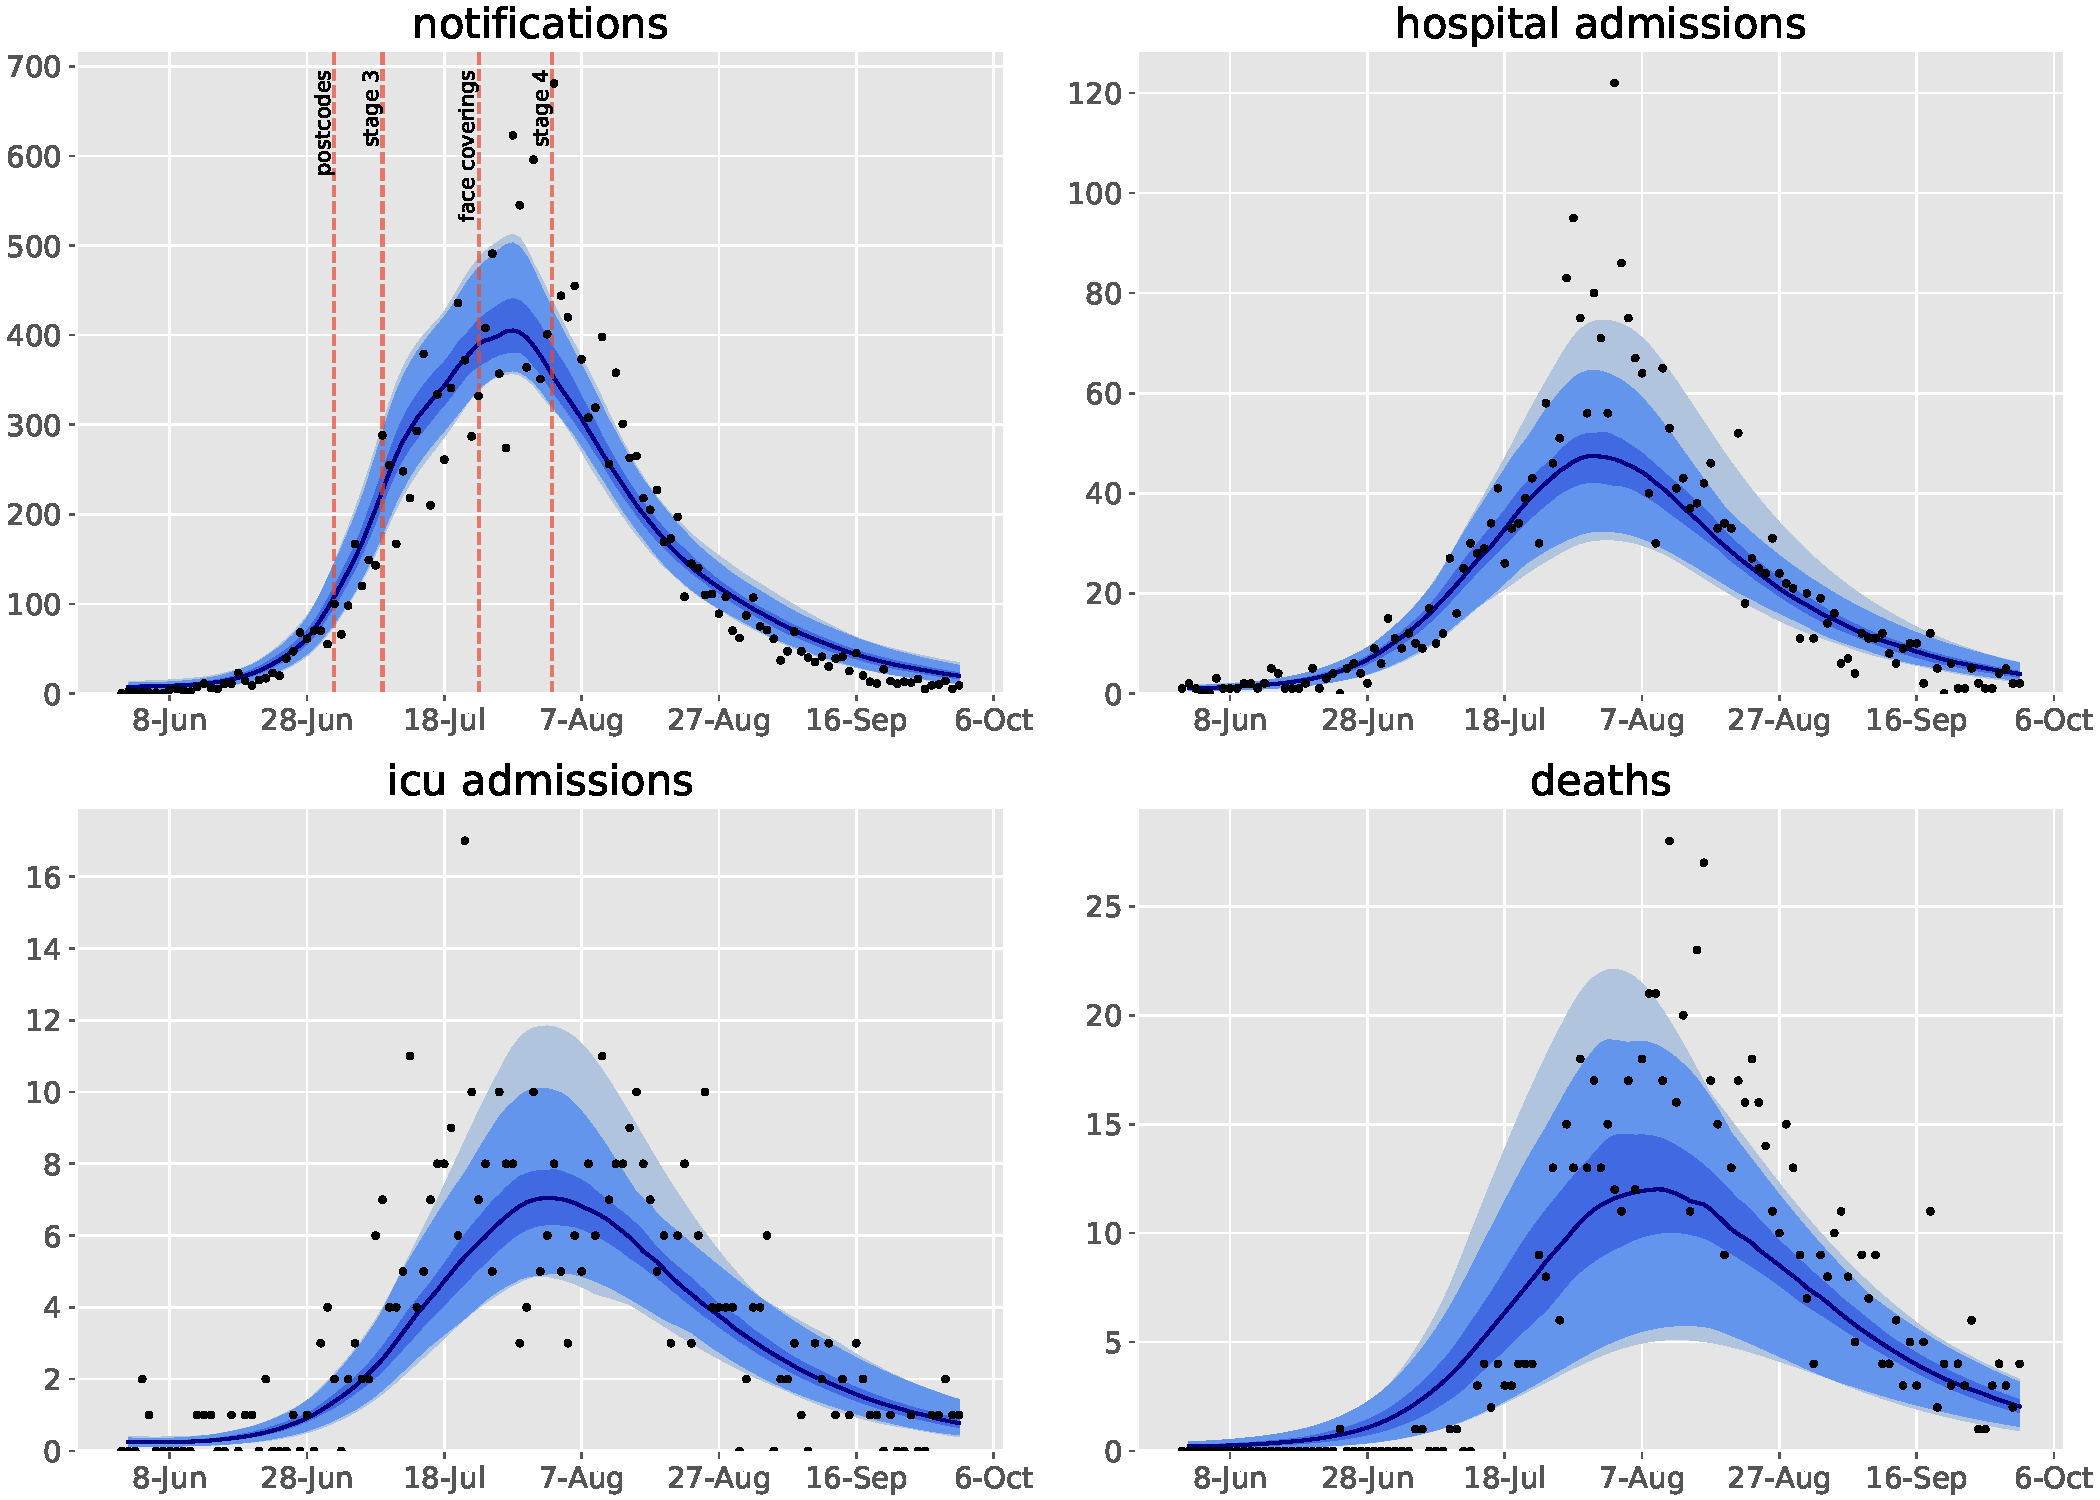
\includegraphics[scale=1]{../covid_19/projects/victoria/prem_sensitivity/multi_output.pdf}}
    \caption{\textbf{Model fit to statewide indicators under sensitivity analysis using matrices from Prem 2020.}}
    \label{fig:prem_sensitivity_outputs}
\end{figure}

\begin{figure}[ht]
    \resizebox{1\textwidth}{!}{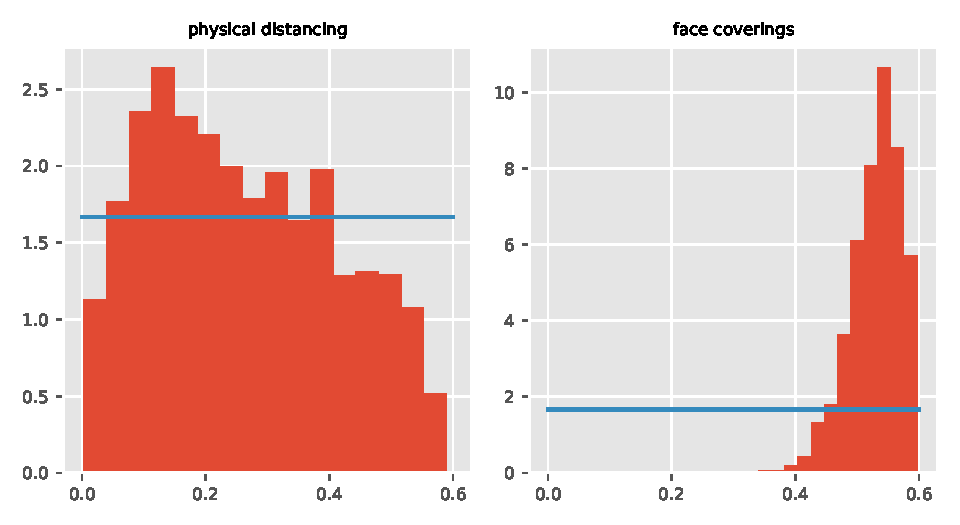
\includegraphics[scale=1]{../covid_19/projects/victoria/prem_sensitivity/key_posteriors.pdf}}
    \caption{\textbf{Posterior distributions of key model parameters under sensitivity analysis using matrices from Prem 2020.}}
    \label{fig:prem_sensitivity_key_params}
\end{figure}

\begin{figure}[ht]
    \resizebox{1\textwidth}{!}{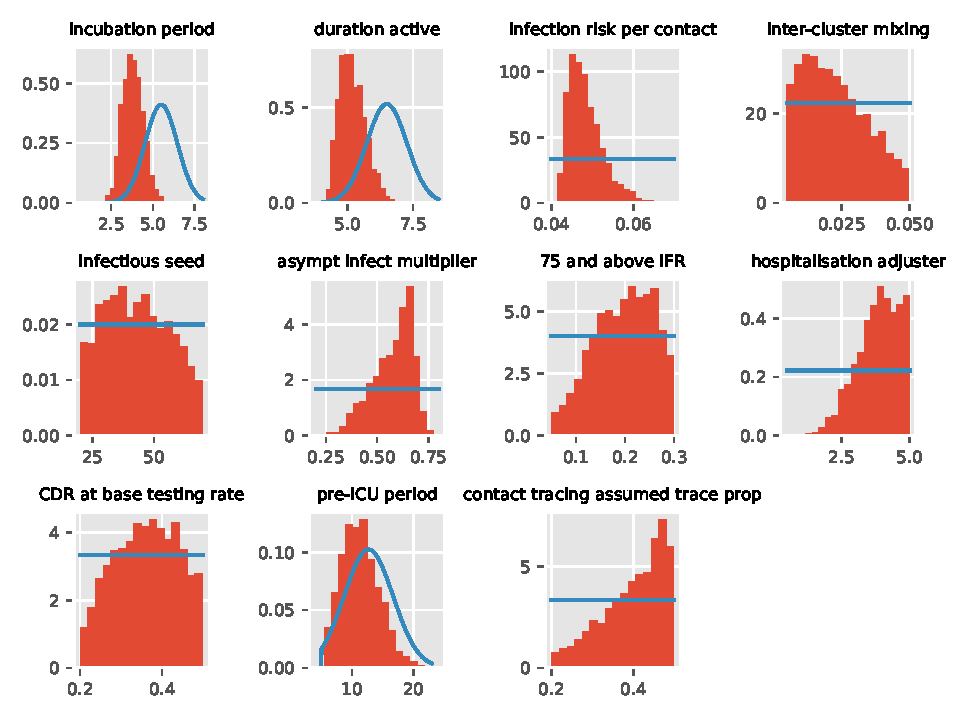
\includegraphics[scale=1]{../covid_19/projects/victoria/prem_sensitivity/epi_posteriors.pdf}}
    \caption{\textbf{Posterior distributions of epidemiological parameters under sensitivity analysis using matrices from Prem 2020.}}
    \label{fig:prem_sensitivity_epi_params}
\end{figure}

\subsection{Sensitivity analysis with Google residential mobility used to scale home location contribution to mixing matrices}
We ran an alternative analysis, in which the home location contribution to the dynamic mixing matrices scaled with Google residential mobility data. This replaced the baseline assumption that the rates of home location contacts remained fixed throughout the simulations. The results of this analysis were similar to that of the baseline analysis and are presented in Figure \ref{fig:residential_sensitivity_outputs}, Figure \ref{fig:residential_sensitivity_key_params} and Figure \ref{fig:residential_sensitivity_epi_params}.

With this approach, the posterior distributions for the incubation period and the duration active shortened well into the lower tail of their respective normal prior distributions. Meanwhile, the effect of face coverings was clustered towards the upper bound of its prior distribution. Exploring the model through manual calibration, the reason for this was determined to be that it was not possible to achieve a sufficiently steep decline in case rates without shortening the serial interval and emphasising the effect of face coverings. This remained the case even if the effect of face coverings was allowed to markedly exceed 50\%. This is because the importance of home contacts increased towards the peak of the epidemic, as Google residential mobility increased. We do not consider this realistic because these contacts would likely have been saturated for those in households with active cases, given that Google residential mobility represents the time spent at home, rather than the number of visits taken to a household. Further, we consider the posterior distributions for the incubation period and duration active too short to be realistic under this model configuration.

\begin{figure}[ht]
    \resizebox{1\textwidth}{!}{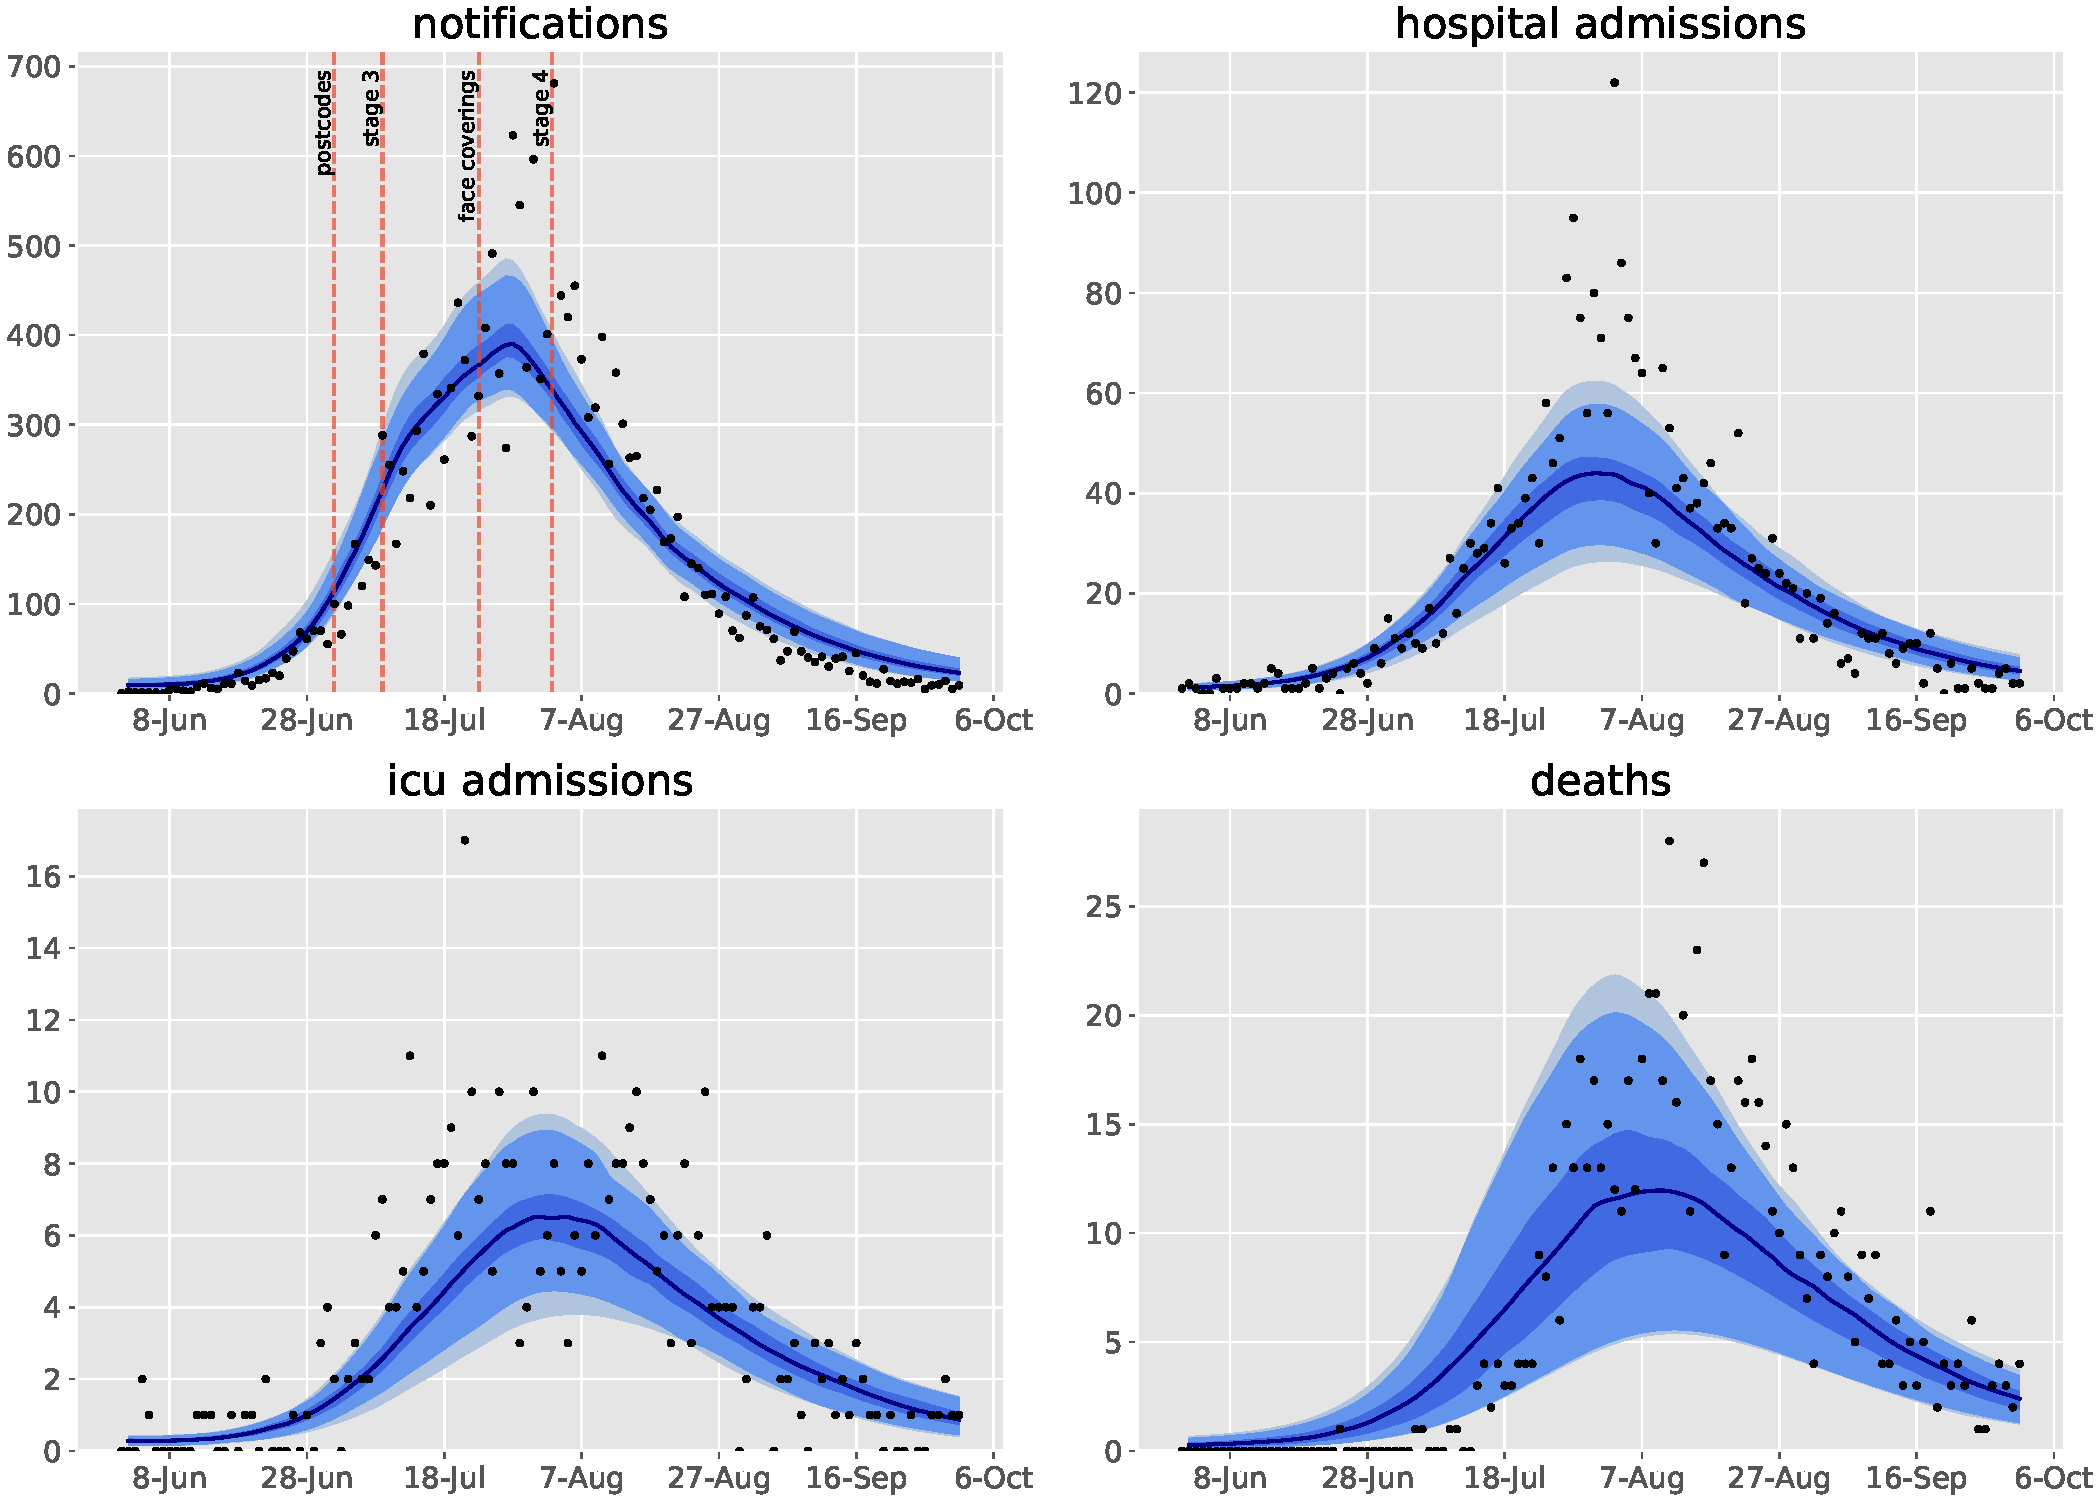
\includegraphics[scale=1]{../covid_19/projects/victoria/home_sensitivity/multi_output.pdf}}
    \caption{\textbf{Model fit to statewide indicators under sensitivity analysis mapping Google residential mobility to home locations of mixing matrices.}}
    \label{fig:residential_sensitivity_outputs}
\end{figure}

\begin{figure}[ht]
    \resizebox{1\textwidth}{!}{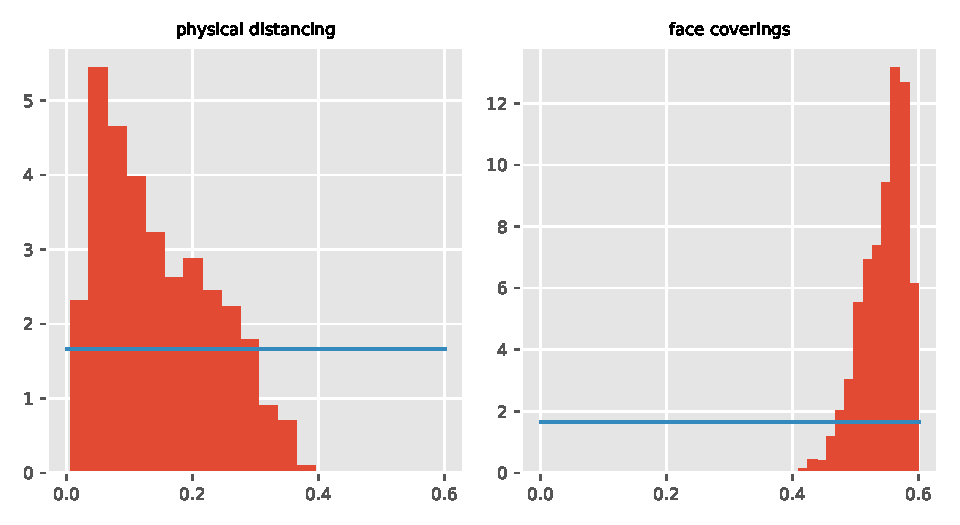
\includegraphics[scale=1]{../covid_19/projects/victoria/home_sensitivity/key_posteriors.pdf}}
    \caption{\textbf{Posterior distributions of key model parameters under sensitivity analysis mapping Google residential mobility to home locations of mixing matrices.}}
    \label{fig:residential_sensitivity_key_params}
\end{figure}

\begin{figure}[ht]
    \resizebox{1\textwidth}{!}{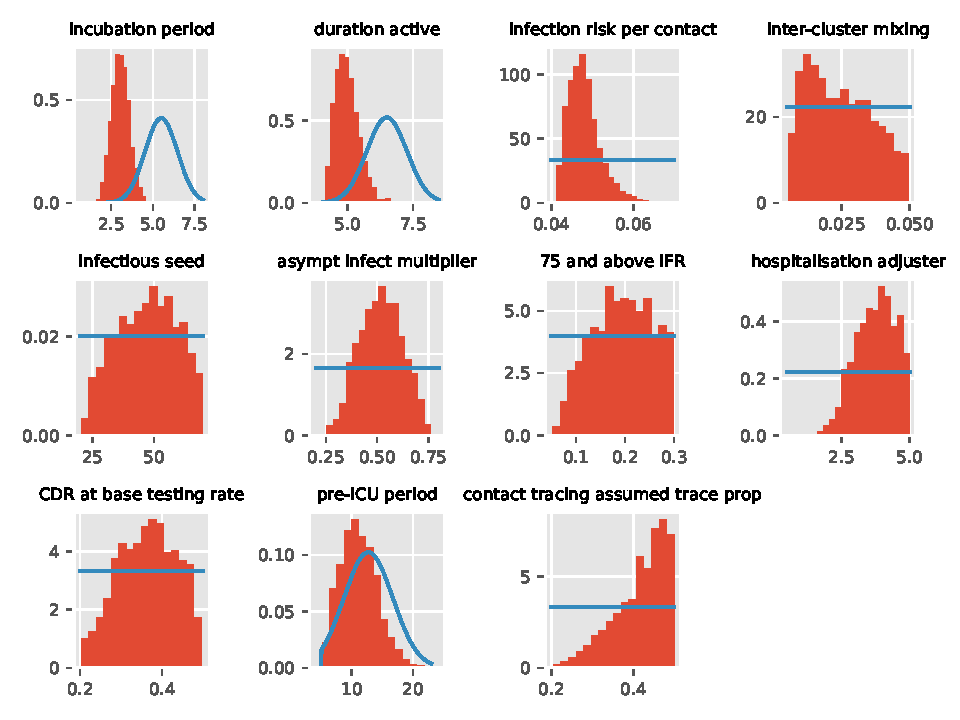
\includegraphics[scale=1]{../covid_19/projects/victoria/home_sensitivity/epi_posteriors.pdf}}
    \caption{\textbf{Posterior distributions of epidemiological parameters under sensitivity analysis mapping Google residential mobility to home locations of mixing matrices.}}
    \label{fig:residential_sensitivity_epi_params}
\end{figure}
